\documentclass[18pt]{beamer}
\usepackage[utf8]{inputenc}
\usepackage[T1]{fontenc}
\usepackage{microtype}
%% SLIDE FORMAT
% use 'beamerthemekit' for standard 4:3 ratio
% for widescreen slides (16:9), use 'beamerthemekitwide'

\usepackage{templates/beamerthemekit}
% \usepackage{templates/beamerthemekitwide}

\usepackage{amsmath}
\usepackage{slashed}
\usepackage{amsfonts}
\usepackage{amssymb}
\usepackage{siunitx}
\sisetup{detect-weight=true, detect-family=true}
\usepackage{color}
%\usepackage{todonotes}
%\presetkeys{todonotes}{i		nline}{}
%\usepackage{booktabs}
\usepackage{listings}
\usepackage[style=numeric, backend=biber, sorting=ynt]{biblatex}


%------additional package-------
\usepackage{slashed}
%------additional package-------


\addbibresource{bibliography.bib}
\beamertemplatenavigationsymbolsempty


\titleimage{Susy}
\titlelogo{kidfriendly} 

% use these packages for PCM symbols and UML classes
% \usepackage{templates/tikzkit}
% \usepackage{templates/tikzuml}


\title[SUSY]{Susanne, Freunde nennen mich Susy}
\author{Moritz Bauer, Jens Schäfer, Benedikt Stolz, Jan van der Linden}

\institute{Institut für Experimentelle Teilchenphysik (ETP)}

% Bibliography
%\usepackage[citestyle=authoryear,bibstyle=numeric,hyperref,backend=biber]{biblatex}

%\addbibresource{templates/example.bib}
%\bibhang1em



\begin{document}

\selectlanguage{ngerman}

%title page
\begin{frame}
\titlepage
\end{frame}


%table of contents
\begin{frame}{Outline}
\tableofcontents
\end{frame}

%--- Jens:
\begin{frame}{SUSY theory}
	\begin{block}{ }
		\begin{itemize}
\item symmetry under spin transformation\\
\item MSSM: model with fewest new particles% but $10^2$ free parameters\\
\item might solve GUTs and explains dark matter\\
\item quarks \& leptons $\rightarrow$ squarks \& sleptons (spin 0)\\
\item gauge bosons $\rightarrow$ gauginos (spin 1/2) 
		\end{itemize}
	\end{block}

	\begin{figure}[B]
		\centering
	 	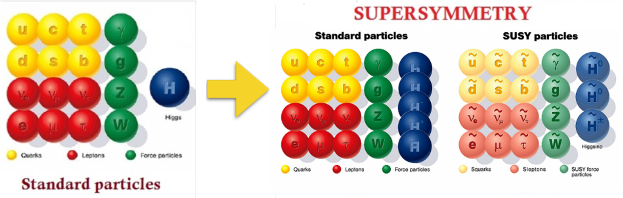
\includegraphics[width=1\textwidth,]{figures/mssm2.png}
		\caption{
			\begin{tiny}
	source:  http://inspirehep.net/record/1407182/files/SUSY.png
			\end{tiny}}
	\end{figure}
\end{frame}

%\begin{frame}{LM6 \& LM9}
%\section{LM6 \& LM9}
%\begin{itemize}
%\item benchmark models leads to different branching %ratios \& behaviours\\
%\item LM6 \& LM9 have relative high cross sections\\ 
%\item SUSY-processes: squark \& gluino pair production
%\end{itemize}

%\begin{figure}[H]
%	\centering
%	 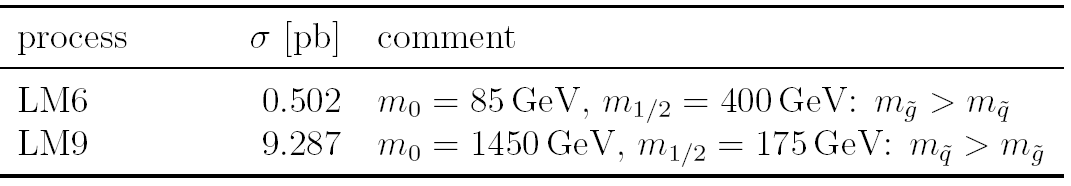
\includegraphics[width=\textwidth,]{figures/properties.png}
	%\caption{aus Übungsblatt Nr. 10}
%\end{figure}

%\end{frame}

\begin{frame}{SUSY phenomenology}
	\begin{block}{  }
		\begin{itemize}
%\item quantum number $R=(-1)^{3B+L+2S} \quad R_{SM}=+1 \qualld R_{SUSY}=-1$ \\
\item conservation of R-parity leads to stable LSP\\
\item LSP is only weak interacting, reconstructable via $\slashed{H}_T$ \\
\item SUSY production: \quad gluino or squark pair production\\
\item SUSY decay: \quad $\tilde{g} \rightarrow q +\tilde{q};\quad  \tilde{q} \rightarrow q + LSP;$\\ 
% \quad leading to high $H_T$ and many jets\\ 
\item expect hadronic signatures with high $H_T, \slashed{H}_T$ and many jets
%$W(l\nu)+jets, Z(\nu\nu)+jets, t\bar{t}+jets, QCD$ 
		\end{itemize}
	\end{block}

	\begin{figure}[H]
	\centering
	 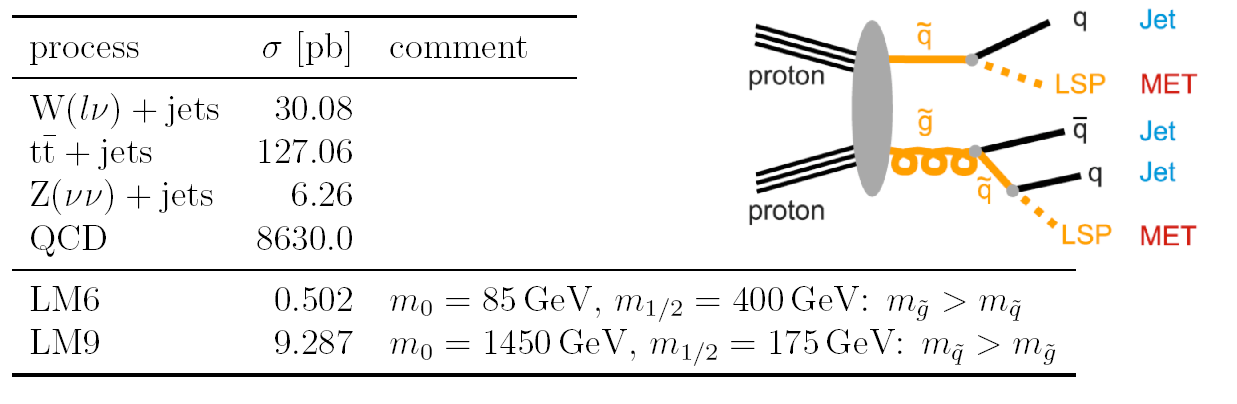
\includegraphics[width=\textwidth,]{figures/feynman+bkg.png}
	\end{figure}
\end{frame}


%----- Ben:

%- Baselinecuts (vor baseline vergleichen mit nach baseline) + Leptonveto

%- Stackedergebnis plot - Susy gefunden? Spoiler: Nein (Zwishcnergebnis)
\begin{frame}
	\frametitle{A first Glance at Data}
	Before analysis the data pre-selection cuts are taken to reduce the amount of data and improve the calculation time of the MC simulation. 
	\begin{block}{Pre-Selection Cuts}
		\begin{itemize}
			\item  $H_T > 300\si{GeV}$ and $N_{\si{jets}} \geq 2$
			\item  $\slashed{H}_T > 100\si{GeV}$ in case of QCD
		\end{itemize}
	\end{block}
	
	\begin{center}
		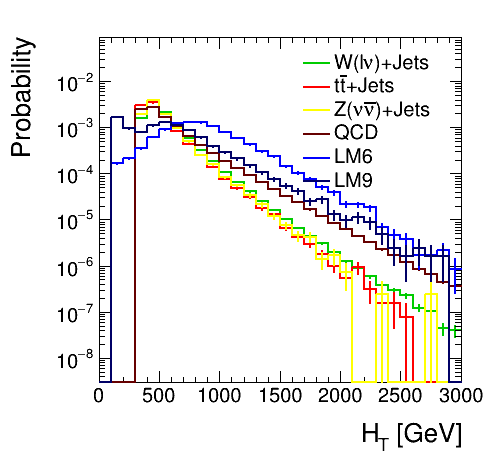
\includegraphics[width = 0.4\textwidth]{plots10/hHt.png}
		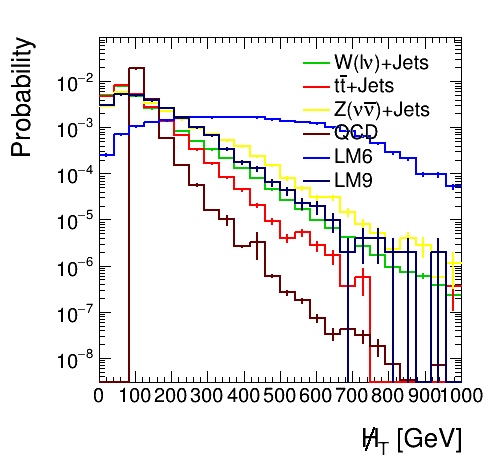
\includegraphics[width = 0.4\textwidth]{plots10/hMht.png}
	\end{center}

\end{frame}

 
\begin{frame}
	\frametitle{Baseline-Cuts}
	\begin{block}{5 Selection Criteria}
		\begin{itemize}
			\item No lepton events with  $p_T > 50 \si{ GeV}$ and $\lvert\eta\rvert < 2.5$ are considered
			\item $N_{\si{jets}} > 3$ with $p_T > 50 \si{ GeV}$ and $\lvert\eta\rvert < 2.4$
			\item $H_T > 500\si{GeV}$ with $p_T > 50 \si{ GeV}$ and $\lvert\eta\rvert < 2.5$
			\item $\slashed{H}_T > 200\si{GeV}$ with $p_T > 30 \si{GeV}$ and $\lvert\eta\rvert < 5.0$	
			\item $\Delta\phi(\si{jet}_{1,2},\slashed{H}_T) > 0.5$ and  $\Delta\phi(\si{jet}_3,\slashed{H}_T) > 0.3$
		\end{itemize}
	\end{block}
	
	\begin{center}
		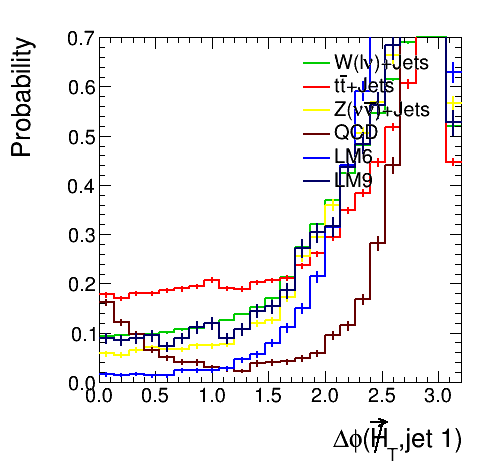
\includegraphics[width = 0.35\textwidth]{plots10/hDeltaPhi1.png}
		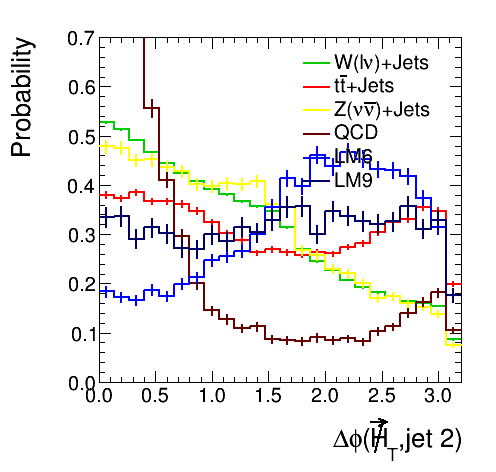
\includegraphics[width = 0.35\textwidth]{plots10/hDeltaPhi2.png}
	\end{center}
	
\end{frame}


\begin{frame}
	\frametitle{Results after applying baseline cuts}
	\begin{block}{background estimation}
		\begin{itemize}
			\item Improved understanding and characterization of background 
			\item QCD-Events are well filtered
			\item No evidence for SUSY-Particles so far
		\end{itemize}
	\end{block}
	
	\begin{center}
		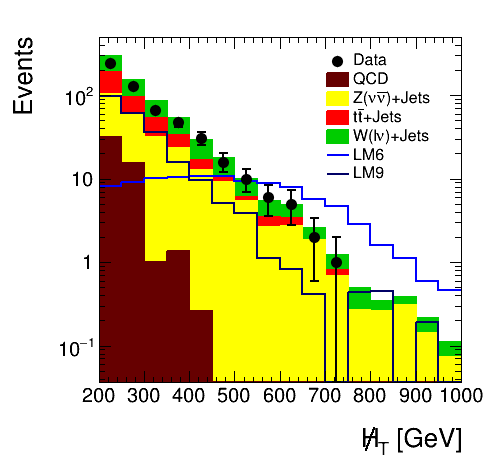
\includegraphics[width = 0.4\textwidth]{plots10/hDataVsMC_Mht.png}
		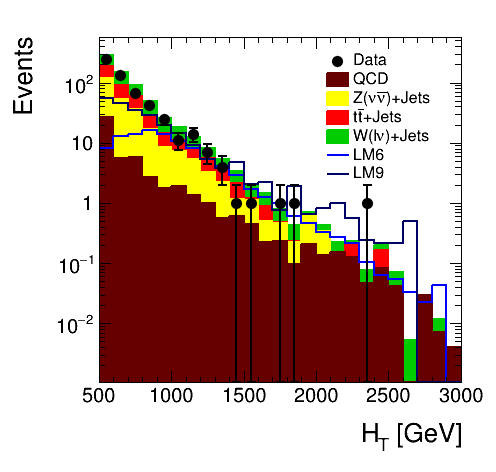
\includegraphics[width = 0.4\textwidth]{plots10/hDataVsMC_Ht.png}
	\end{center}

\end{frame}
%----- Moritz:

%- Wie kommt man an die Gewichte der Events? -> data driven bkg estimation

%- lost lepton  

\begin{frame}
  \frametitle{Data-driven background estimation}
  \begin{itemize}
    \item Use data instead of MC to get lower uncertainties
    \item Example: Use Z($\mu \mu$) + jets and replace muons with neutrinos
    \item Disadv.: $\mathcal{B}(Z \rightarrow \mu \mu) < \mathcal{B}(Z \rightarrow \nu \nu)$ increases stat. uncertainty 
  \end{itemize}
  \begin{figure}[H]
    \centering
    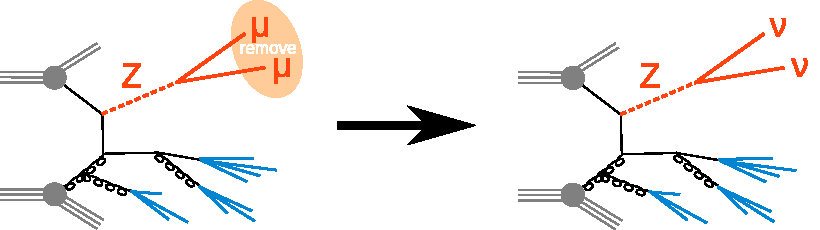
\includegraphics[width=0.8\textwidth]{figures/zmumu}
  \end{figure}
\end{frame}

\begin{frame}
  \frametitle{MC-only background estimation}
  \begin{figure}[H]
    \centering
    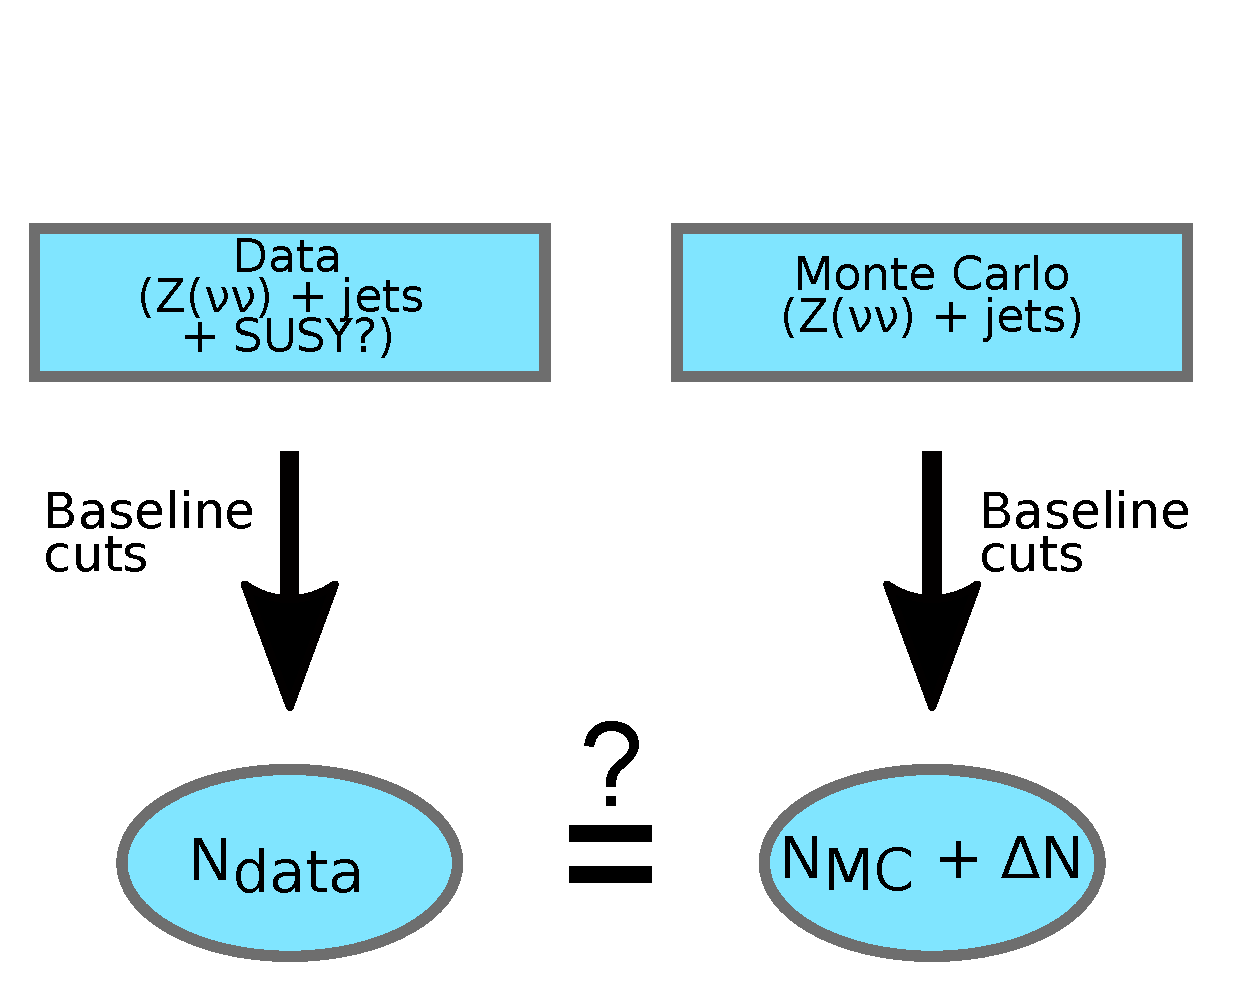
\includegraphics[width=0.7\textwidth,height=0.7\textheight,keepaspectratio]{figures/mc_znunu}
  \end{figure}
\end{frame}

\begin{frame}
  \frametitle{Data-driven background estimation (with Z($\mu\mu$))}
  \begin{figure}[H]
    \centering
    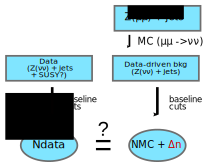
\includegraphics[width=0.8\textwidth,height=0.8\textheight,keepaspectratio]{figures/ddbe_zmumu}
  \end{figure}
\end{frame}

\begin{frame}
  \frametitle{Lost-lepton estimation}
  \begin{itemize}
    \item Lost leptons are electrons/muons not removed by lepton veto
    \item Reasons: Lepton not accepted, not well-reconstructed or not isolated
    \item Different approach is needed here: data-driven background estimation
  \end{itemize}

  \begin{figure}[H]
    \centering
     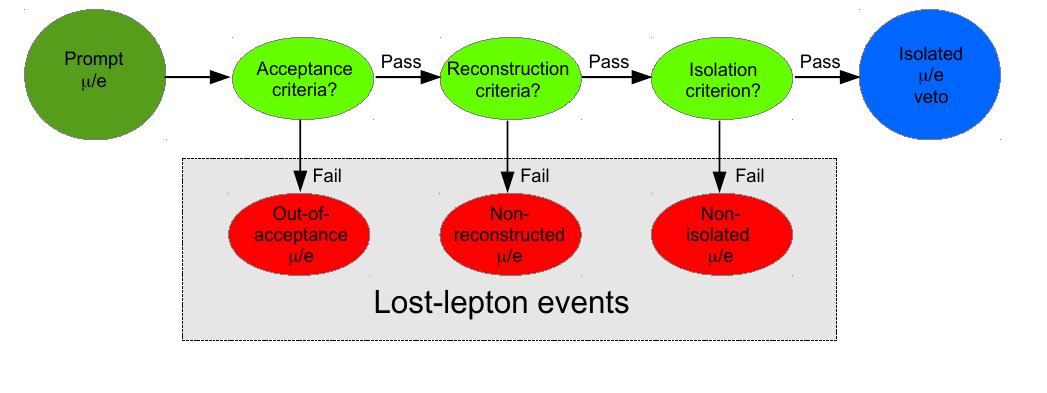
\includegraphics[width=\textwidth]{figures/lost-lepton.png}
    %\caption{aus Thesis}
  \end{figure}

\end{frame}

\begin{frame}
  \frametitle{Data-driven background estimation}
  \begin{itemize}
    \item Goal: Calculated a lost-lepton probability $\omega(\alpha, \epsilon_{reco}, \epsilon_{iso})$ which can be used to weigh the generated events
    \begin{itemize}
      \item $\alpha$: acceptance
      \item $\epsilon_{reco}$: reconstruction efficiency
      \item $\epsilon_{iso}$: isolation efficiency
    \end{itemize}
  \end{itemize}

\end{frame}

%----- Jan:

%- gewichtung motivieren

\begin{frame}{Acceptance/Efficiency Maps}

\begin{block}{Muon Acceptance}
\begin{itemize}
\item evaluated in $N(\si{jets})$- and $\slashed H_{\si{T}}$-bins
\item acceptances highly dependant on bin
\end{itemize}
\end{block}

\begin{center}
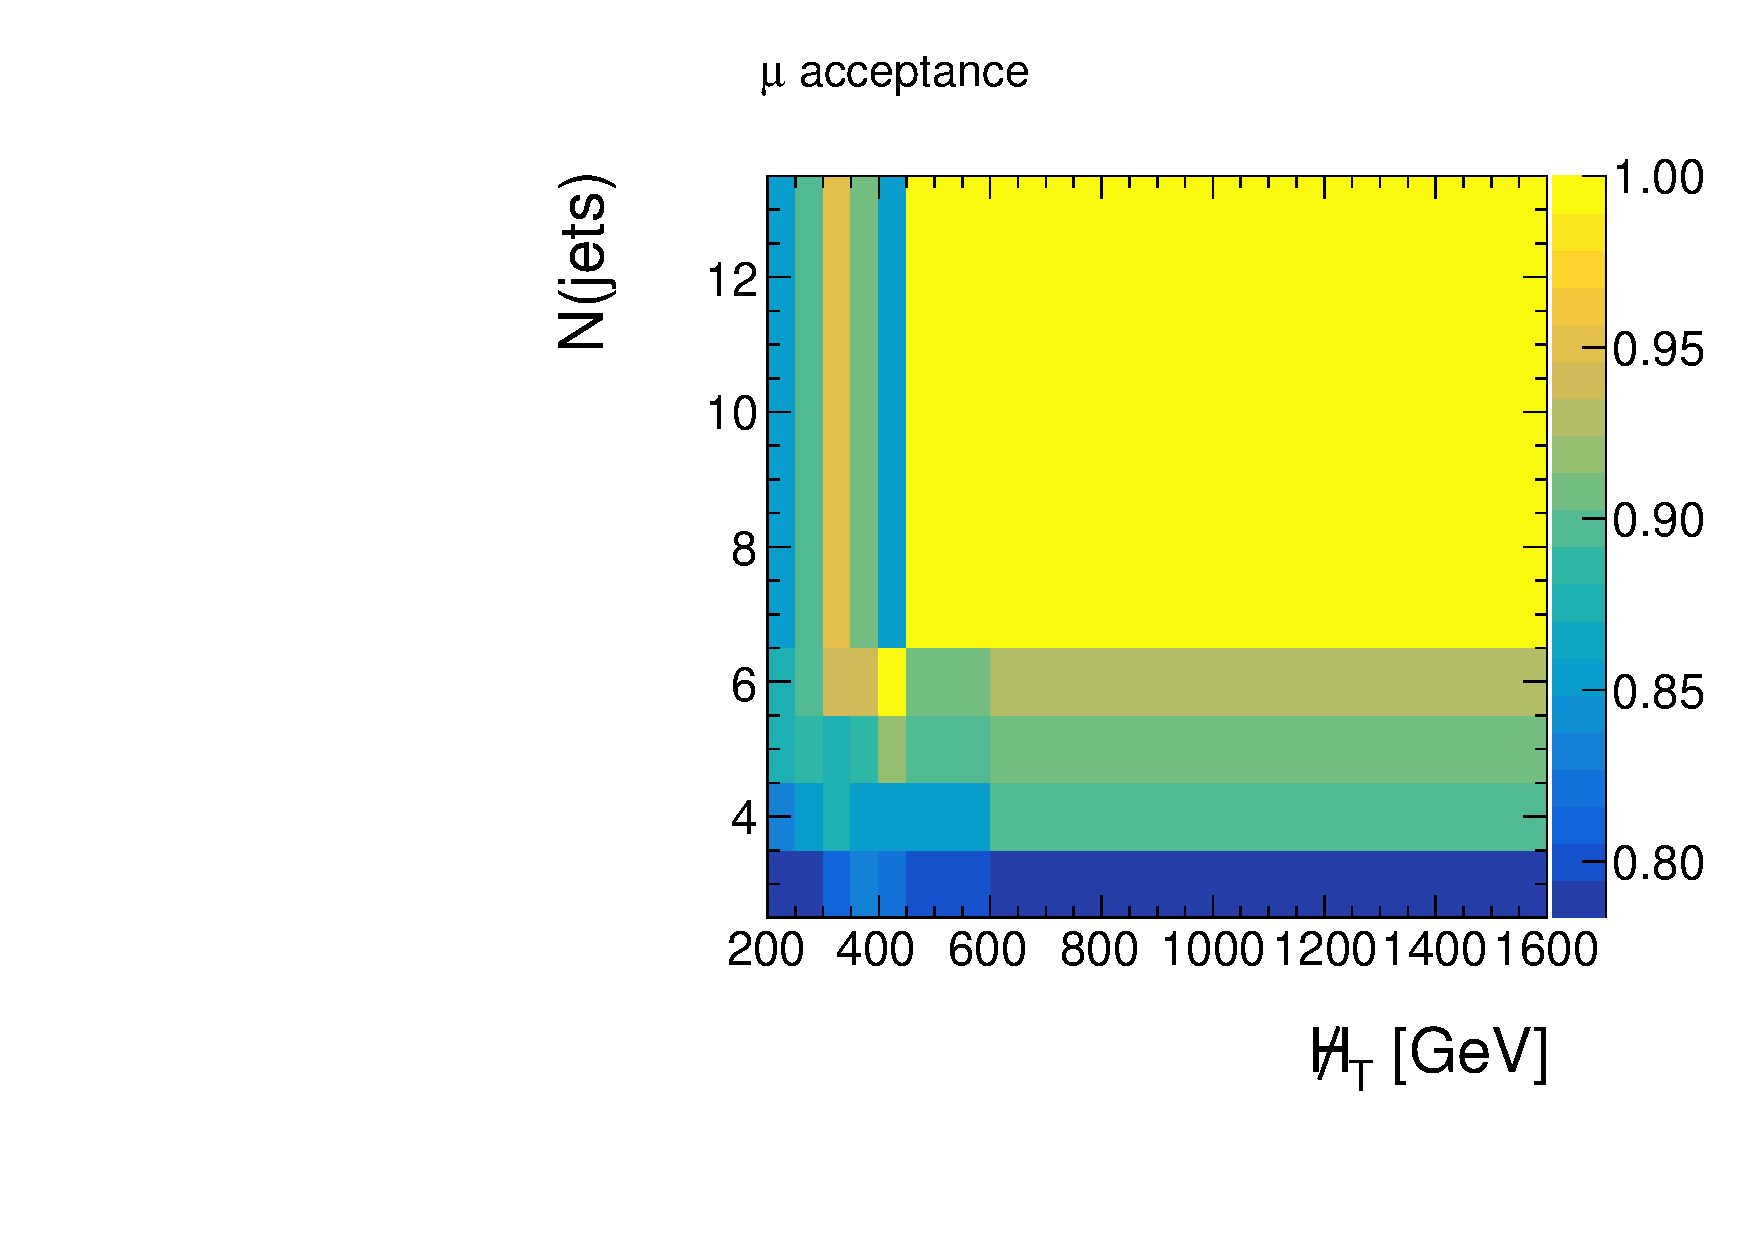
\includegraphics[width = 0.5 \textwidth]{plots11/MuonAcceptance.pdf}
\end{center}

\end{frame}


\begin{frame}{Acceptance/Efficiency Maps}

\begin{block}{Reconstruction Efficiency}
\begin{itemize}
\item only events that pass muon acceptance are considered
\item evaluated in $N(\si{jets})$-, $H_{\si{T}}$- and $\slashed H_{\si{T}}$-bins
\item efficiencies also highly dependant on bin
\end{itemize}
\end{block}

\begin{center}
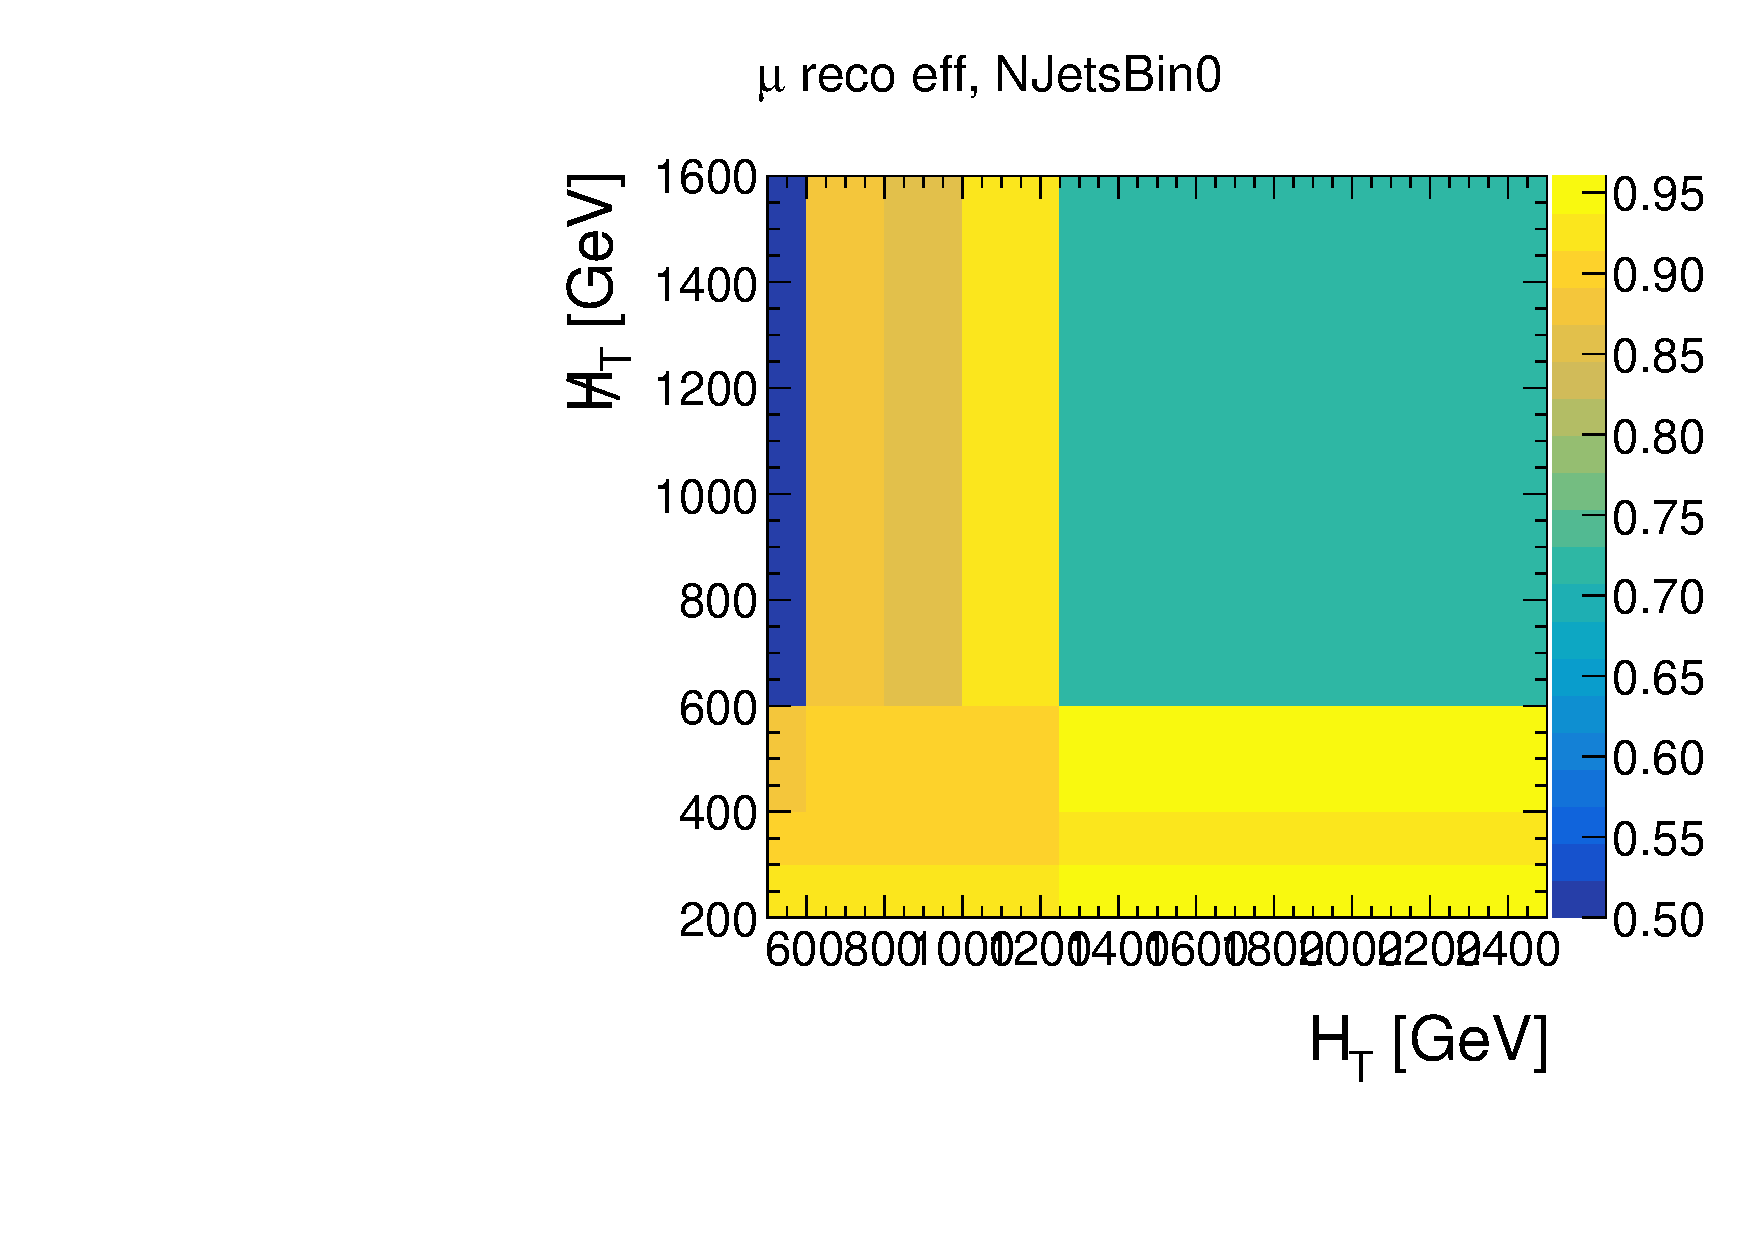
\includegraphics[width = 0.4\textwidth]{plots11/MuonRecoEff_NJetsBin0.pdf}
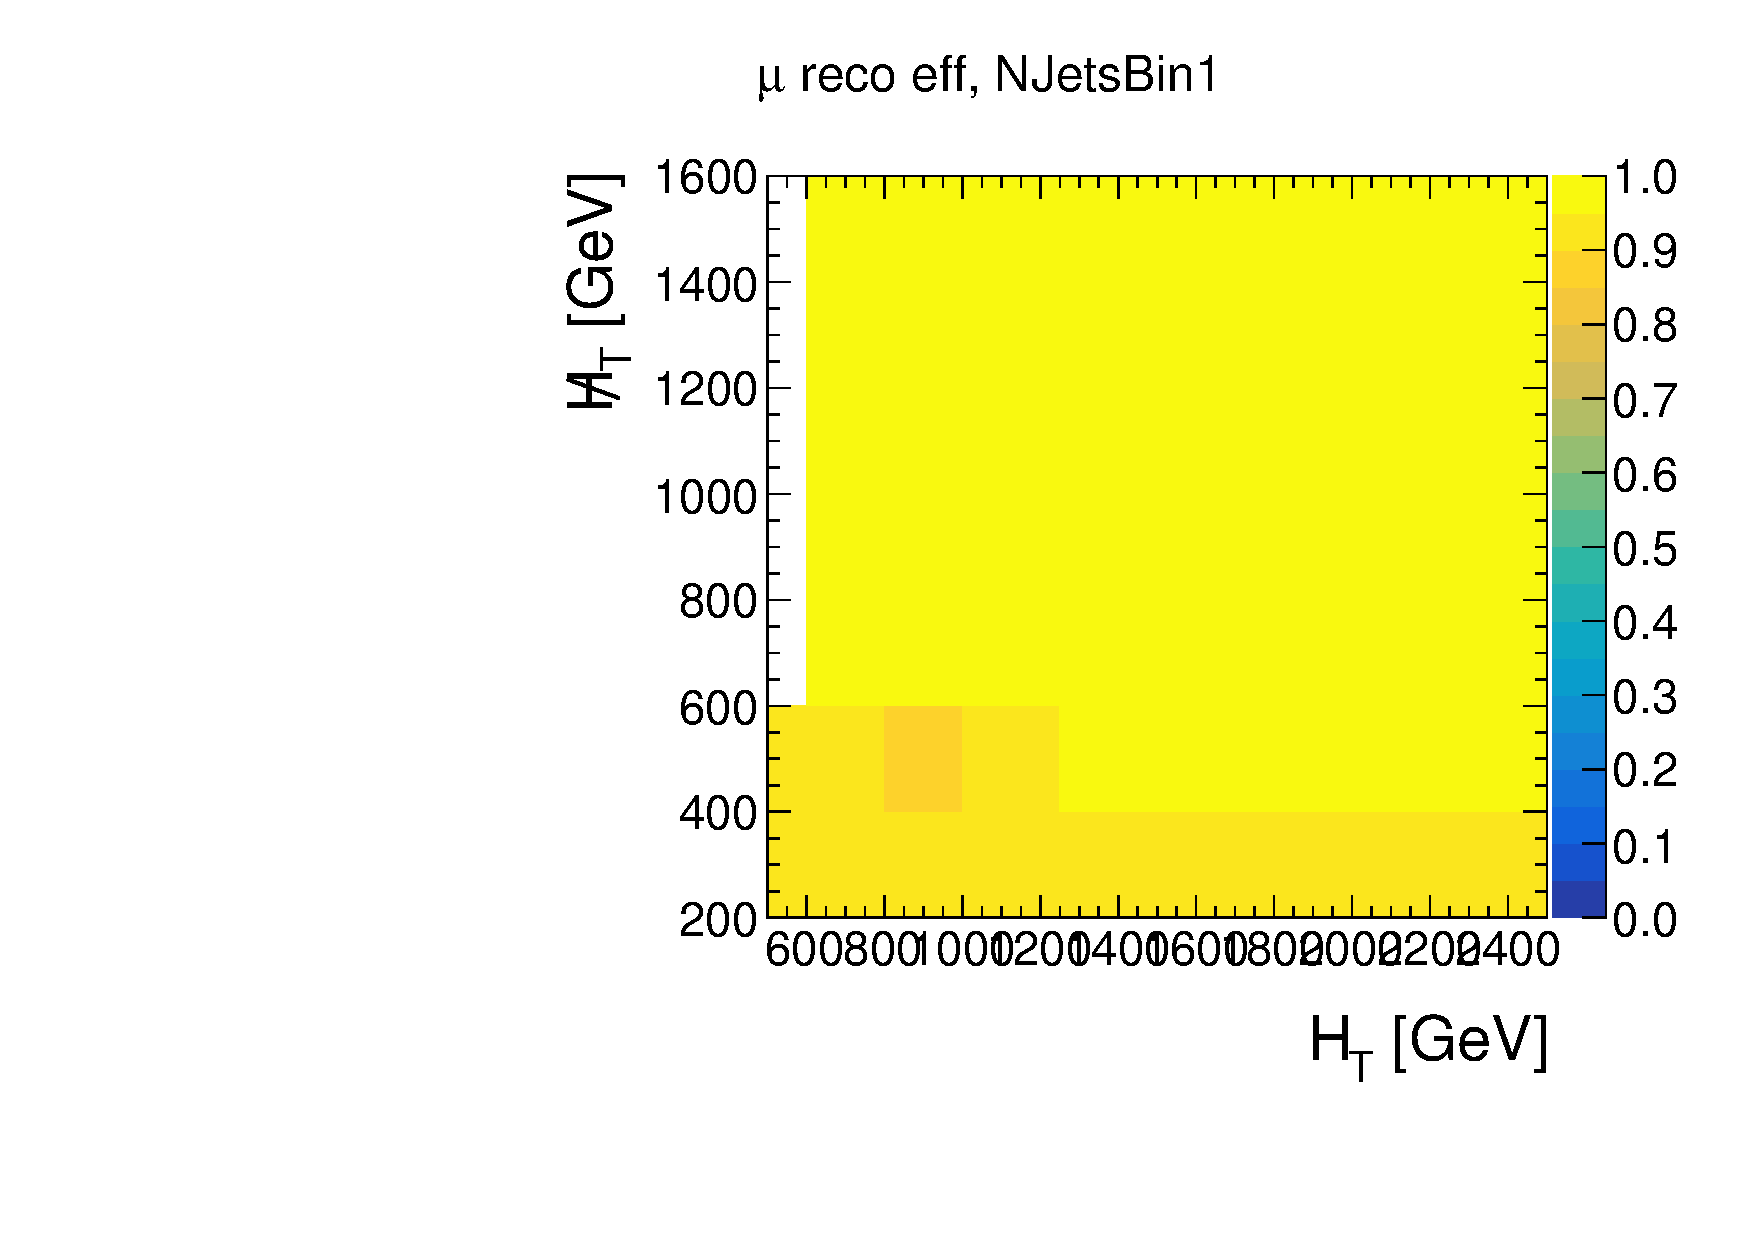
\includegraphics[width = 0.4\textwidth]{plots11/MuonRecoEff_NJetsBin1.pdf}
\end{center}

\end{frame}


%- closure test
\begin{frame}{Validation of the Implemented Method}

\begin{block}{Closure Test}
\begin{itemize}
\item apply self-implemented method to W+jets MC sample\\
\begin{itemize}
	\item cut sample to events with one isolated $\mu$ (control sample)
	\item weight events with probability that $\mu$ is not isolated\\
	$\Rightarrow$ mimic distribution where no isolated $\mu$ found 
\end{itemize}
\item compare to sample where falsely no isolated $\mu$ was found
\end{itemize}
\end{block}

\begin{center}
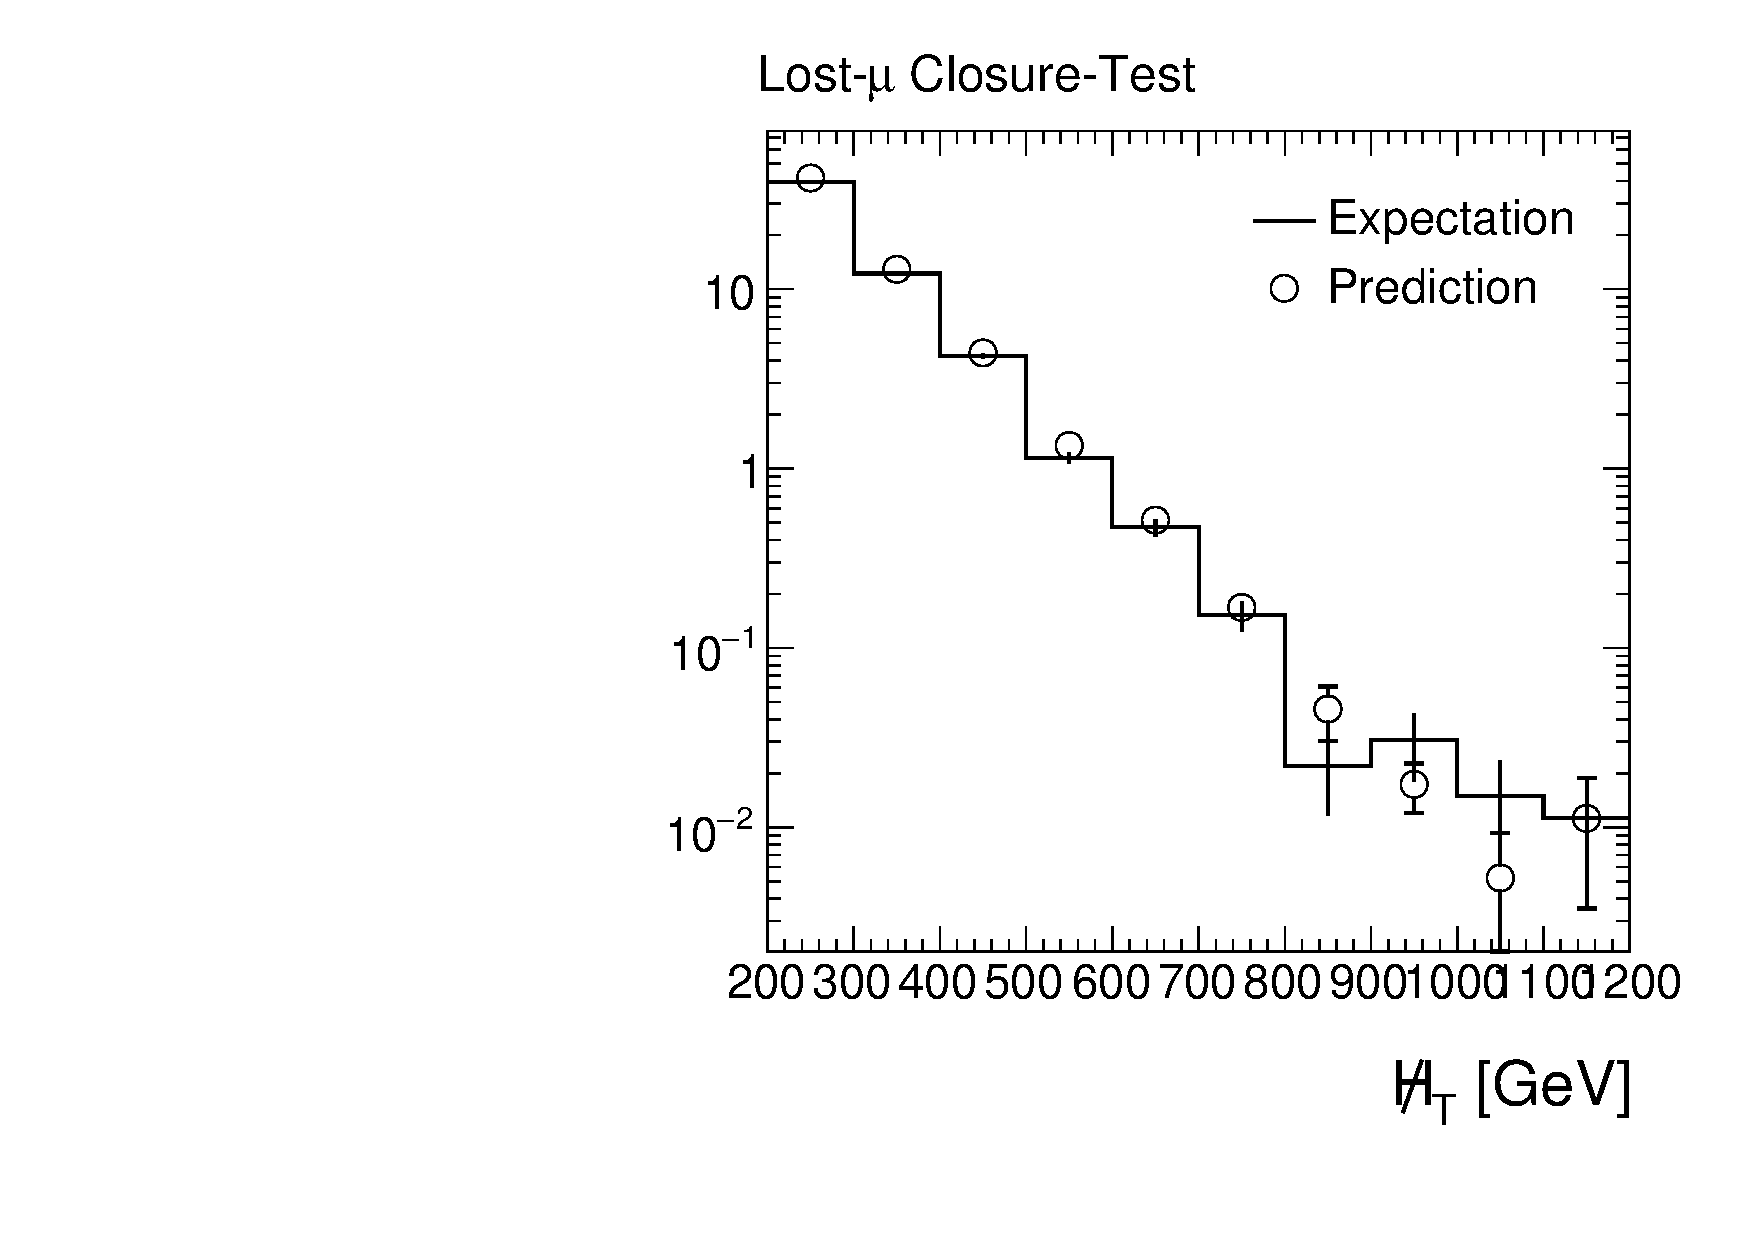
\includegraphics[width = 0.37\textwidth]{plots11/LLClosureMHT.pdf}
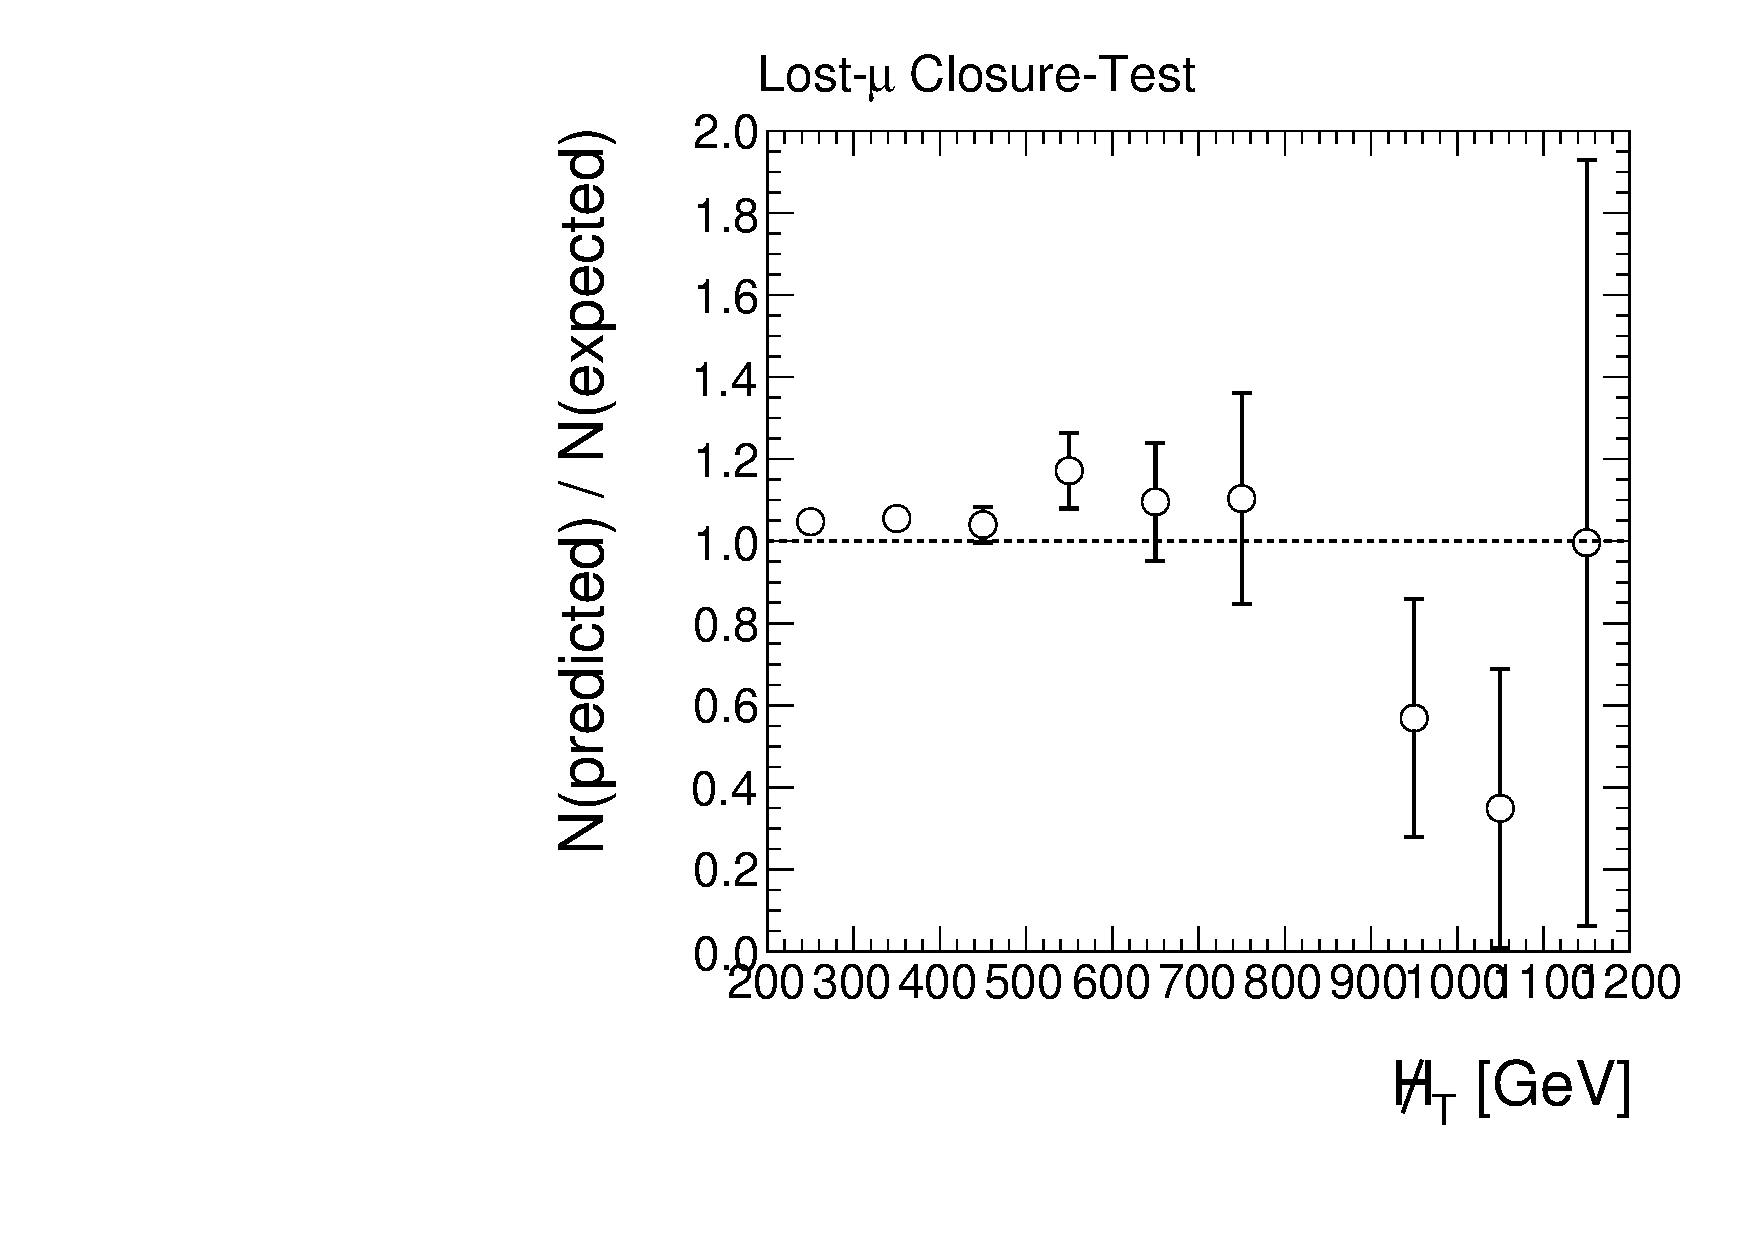
\includegraphics[width = 0.37\textwidth]{plots11/LLClosureMHTRatio.pdf}
\end{center}

\end{frame}


\begin{frame}{Predict Background from Data}

\begin{block}{Method}
\begin{itemize}
\item generate new efficiency maps for full lost-lepton method
\begin{itemize}
	\item consider lost electrons
	\item consider $\mathsf{t\overline{t}}$+jets events
\end{itemize}
\item apply efficiency weighting to data
\end{itemize}
\end{block} 

\begin{center}
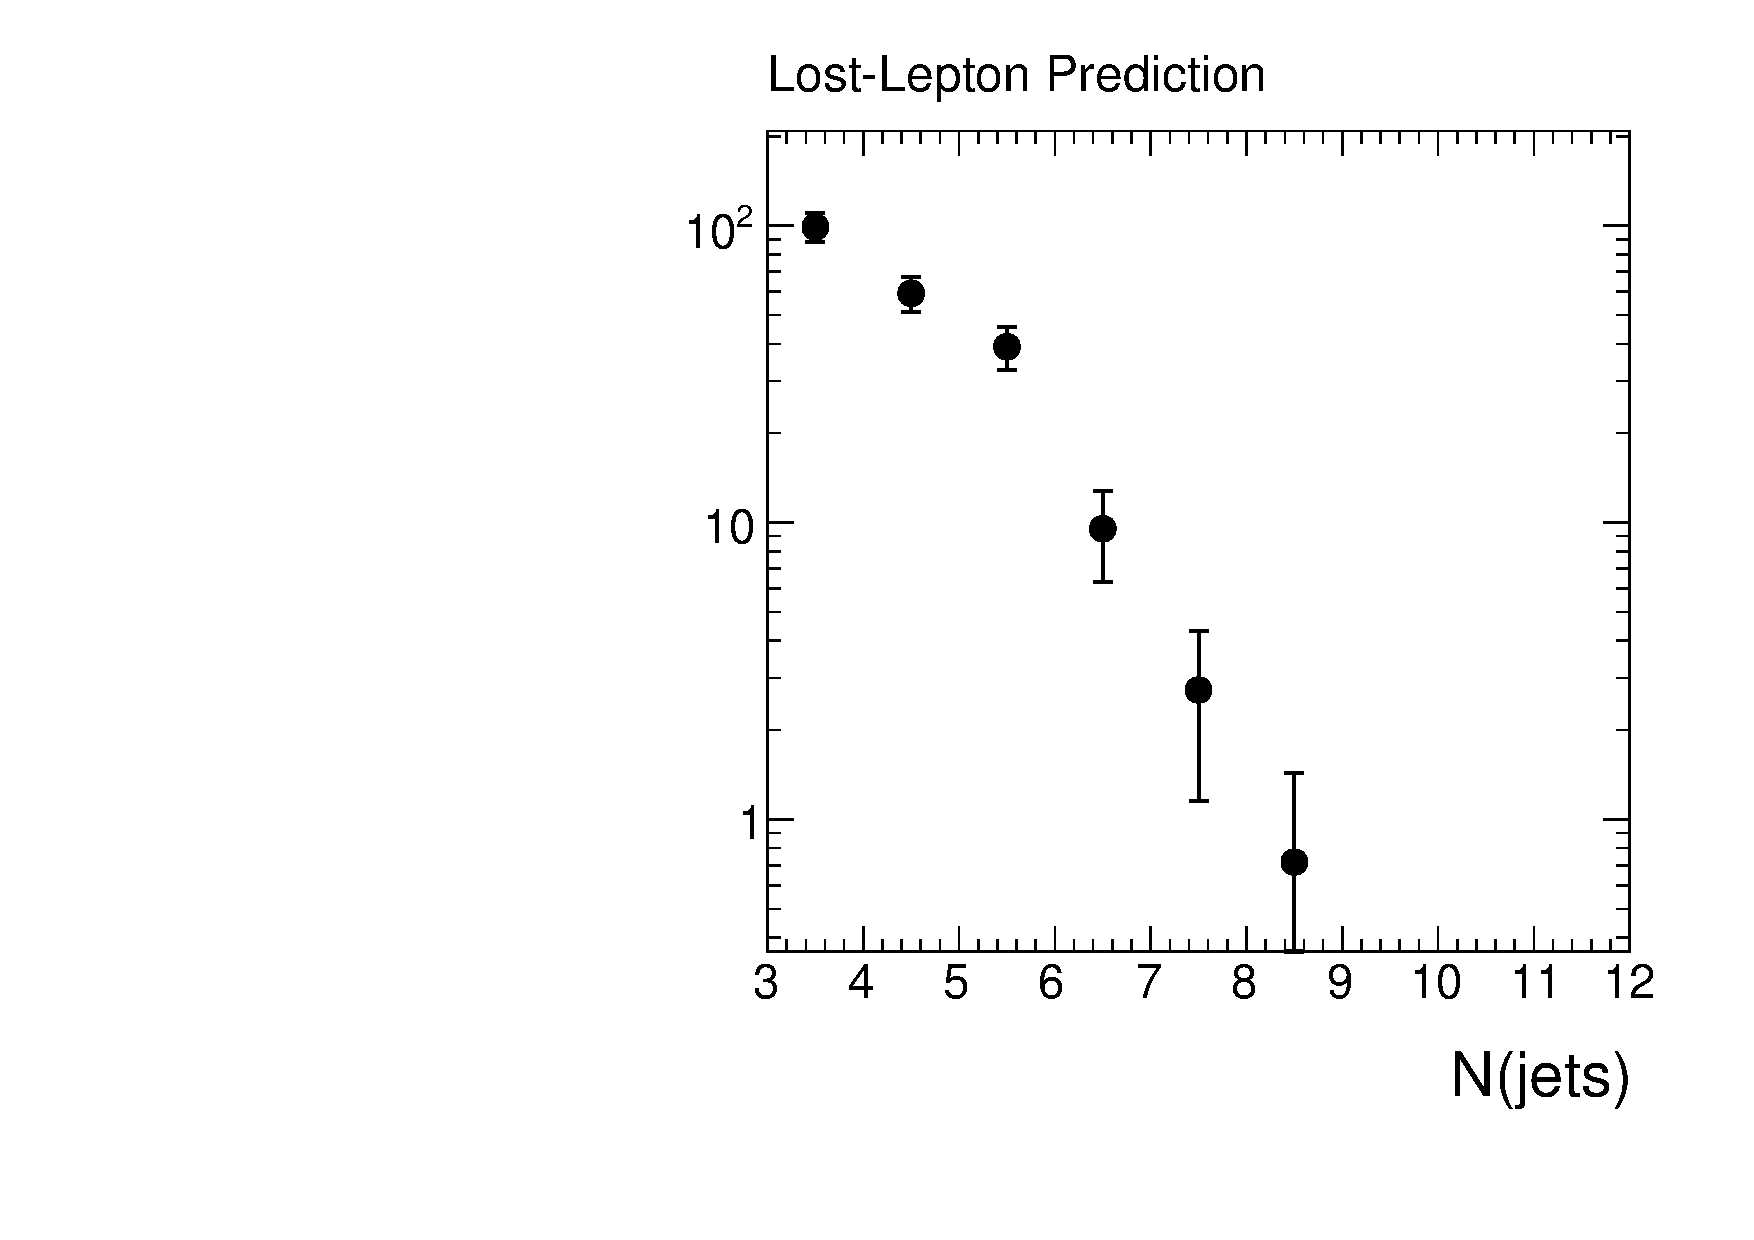
\includegraphics[width = 0.4\textwidth]{plots11/LLPredictionNJets.pdf}
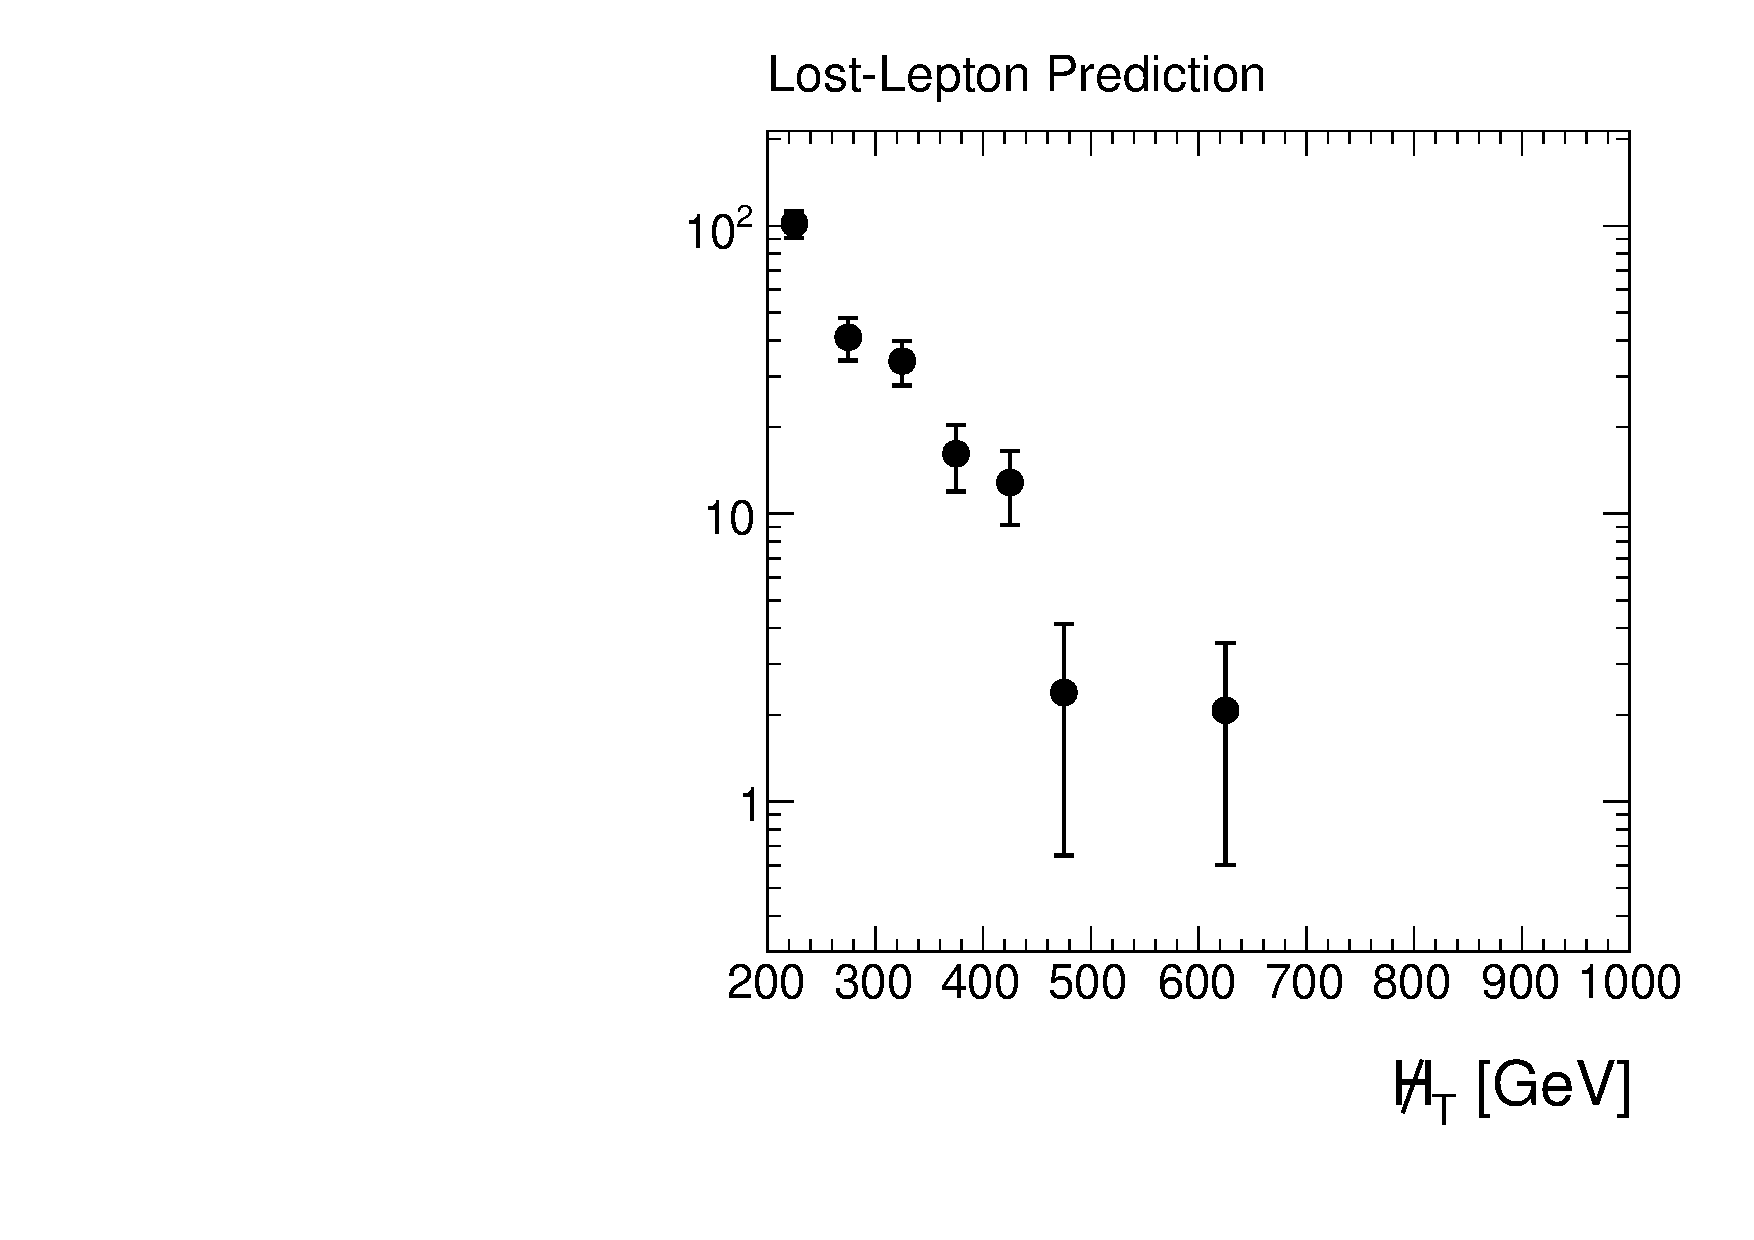
\includegraphics[width = 0.4\textwidth]{plots11/LLPredictionMHT.pdf}
\end{center}

\end{frame}



%- "neues" Ergebnis vs altes (spoiler: Gleich mit homemade gewichten) 
\begin{frame}{Combined Results}

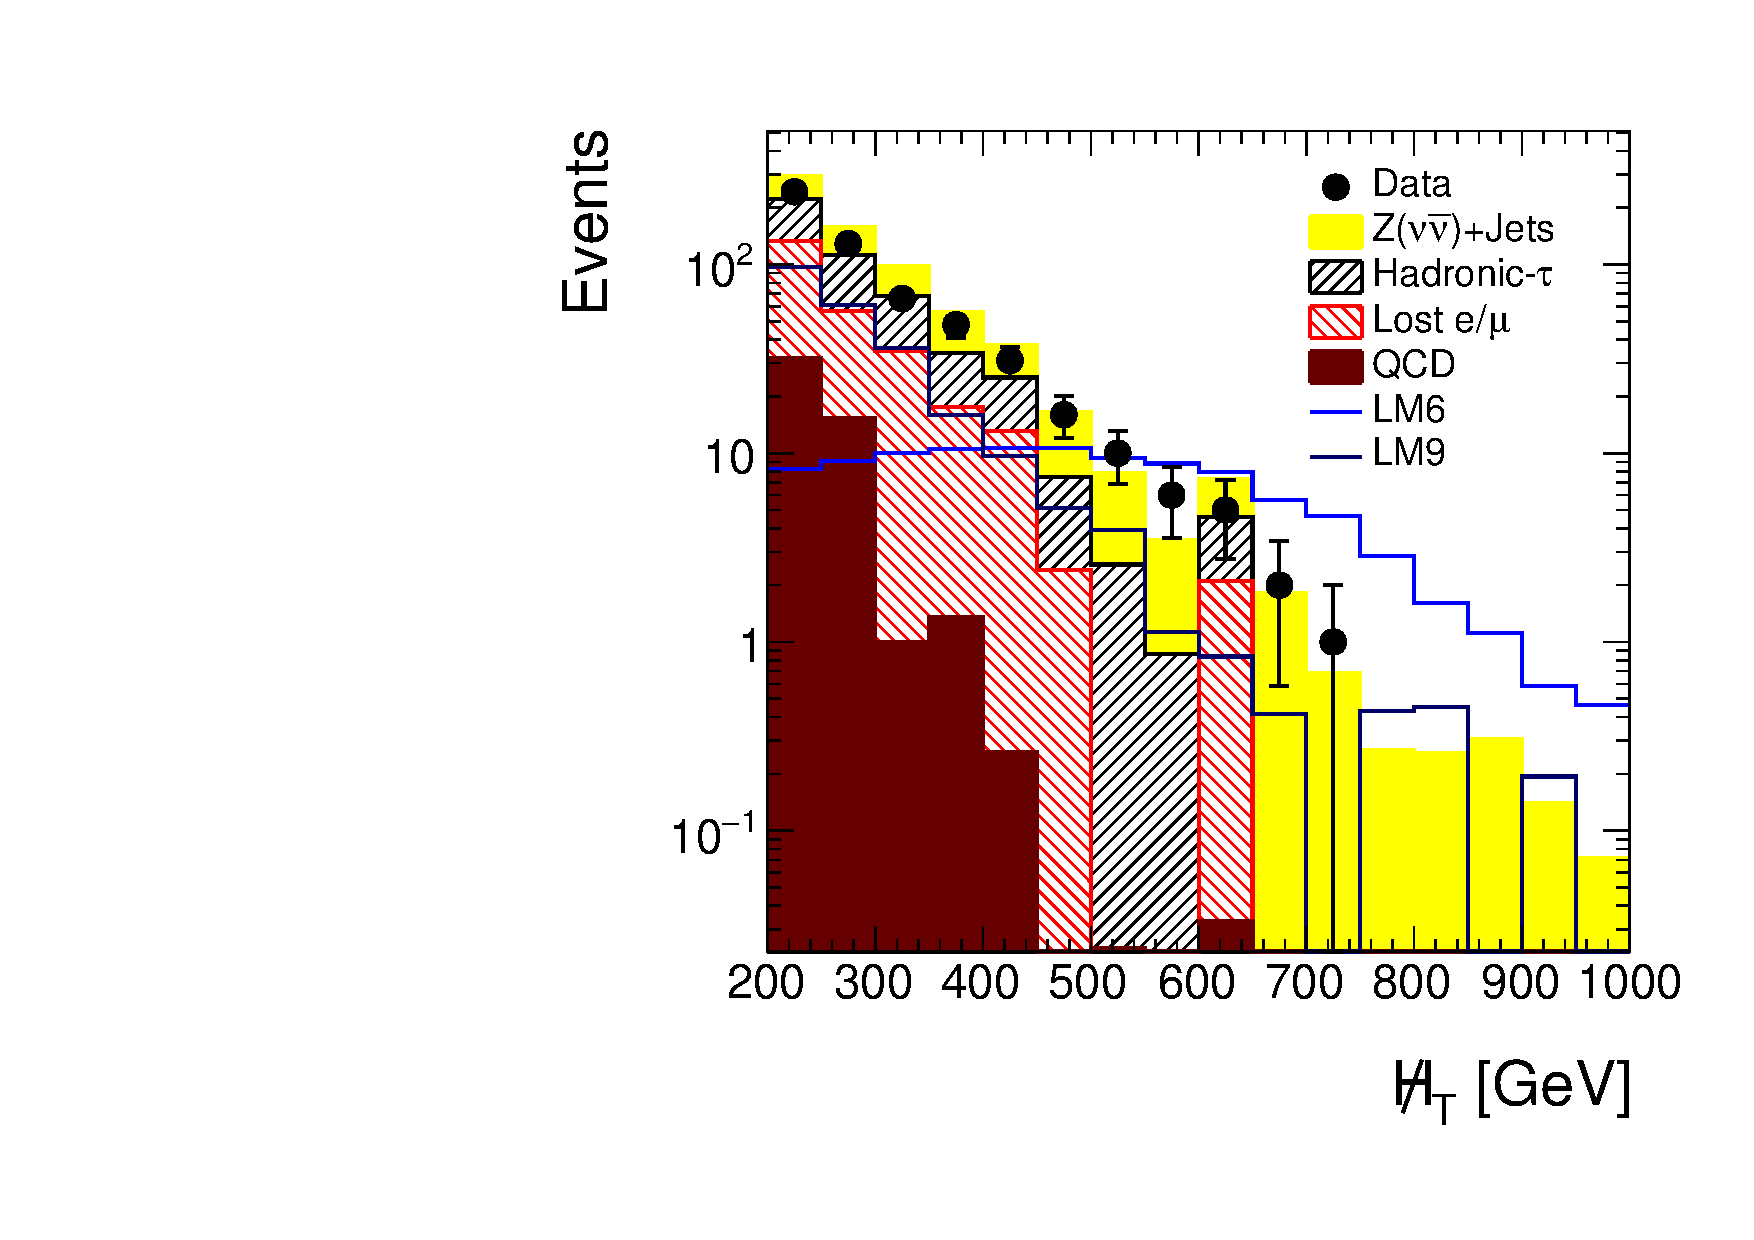
\includegraphics[width = 0.45\textwidth]{plots11/hDataVsBkg_Mht.pdf}
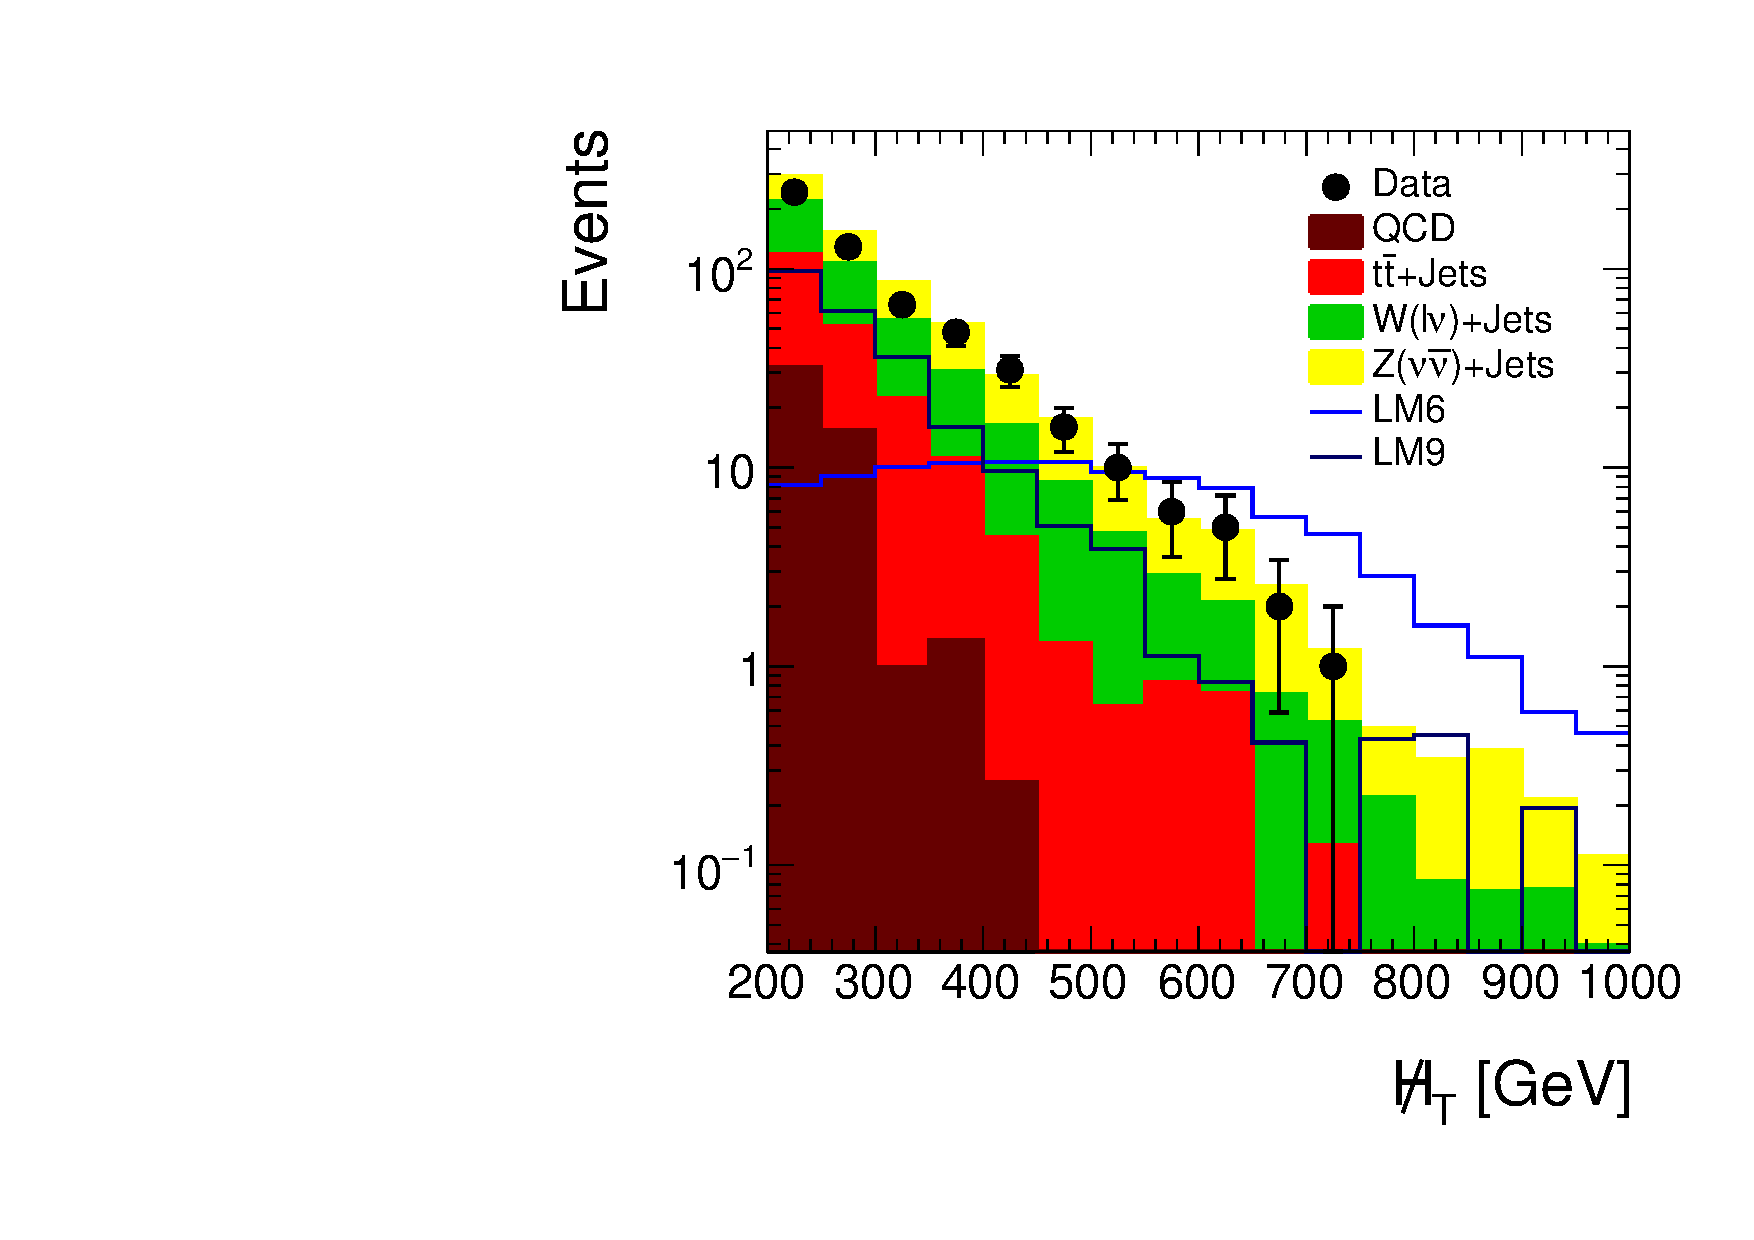
\includegraphics[width = 0.45\textwidth]{plots11/hDataVsMC_Mht.pdf}\\
$\Rightarrow$ still no SUSY found :(
\end{frame} 


\end{document}

